\documentclass{article}

\begin{document}

\setlength{\parindent}{6ex}

\begin{figure}
    \centering
    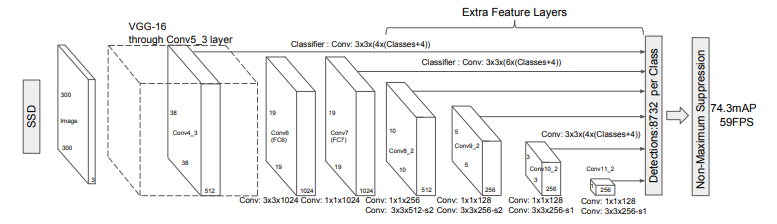
\includegraphics[width=1.25\textwidth]{models/ssd}
    \caption{Network of SSD}
    \label{fig:ssd1}
\end{figure}

\indent

Single Shot MultiBox Detector is a single deep neural network which aims to detect 
objects in real-time. The main improvement in speed comes from eliminating region 
proposals as Faster R-CNN does. Although eliminating region proposals increases 
the speed of detection, it reduces the accuracy significantly. Thus, three main 
improvements are applied to increase accuracy:

\begin{enumerate}
    \item Multi-Scale Feature Maps for Detection
    \begin{itemize}
        \item As mentioned in section 2.3, handling multi-scale is important feature 
for object detectors. It can reduce the mAP for detector's performance since objects 
of different sizes in given image cannot be detected well. To handle multi-scale detection, 
SSD uses multi-scale feature maps instead of using different sizes of input images. 
The size of feature maps decreases through the network's architecture. You can see in figure 
\ref{fig:ssd1} the SSD architecture in which layers are getting smaller from left to right and 
each of these convolutional layers are connected to the prediction module, so that, multi-scale 
feature maps can be used in prediction. For larger feature maps, SSD can detect smaller objects 
and for smaller feature maps, smaller objects can be detected. You can see in figure 
\ref{fig:featmapssd1}, detecting cat in image is done by 8x8 feature map, although, detecting 
dog is done by 4x4 feature map.
    \end{itemize}
    \item Convolutional Predictors for Detection
    \begin{itemize}
        \item Small-size convolutional filters are used to make prediction for 
object detection. These convolutional filters are applied on extracted feature maps 
to compute both localization and class scores. Each filter computes a bounding box and 
corresponding class scores for each category.
    \end{itemize}
    \item Default Bounding Boxes and Aspect Ratios
    \begin{itemize}
        \item SSD divides its feature maps into a grid and each feature map cells are 
associated with a set of default bounding boxes. These bounding boxes have fixed position 
relative to its corresponding grid cell. The aim of using multiple bounding boxes 
in each grid cell is to detect different-shape objects such as cars and people. You can see in 
figure \ref{fig:ssdbbox1}, there are four different bounding boxes for each grid cells. These bounding 
boxes are shaped different than the others to increase the chance of detection of different-shaped 
objects. For example, bounding box 1 in figure \ref{fig:ssdbbox1} can be used to detect cars but 
bounding box 3 is better option for detecting people.
        \item For different layers of SSD, default bounding boxes are customized for 
different resolutions. There are target aspect ratios and corresponding to these 
aspect ratios, default bounding boxes are calculated.
    \end{itemize}
\end{enumerate}

\begin{figure}
    \centering
    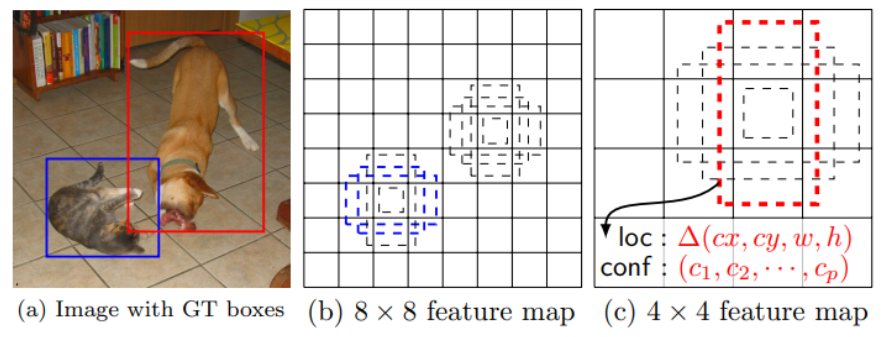
\includegraphics[width=\textwidth]{featmapssd}
    \caption{Multi-scale feature maps}
    \label{fig:featmapssd1}
\end{figure}

\begin{figure}
    \centering
    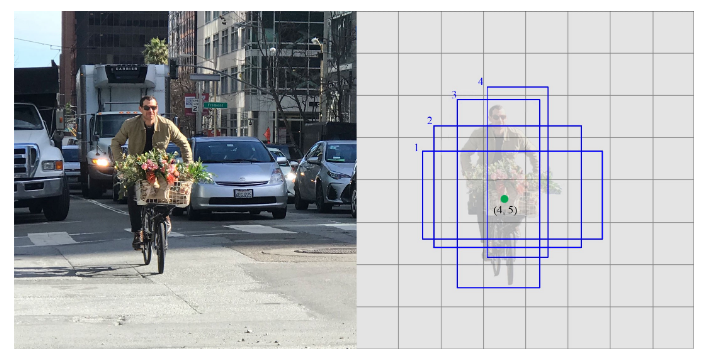
\includegraphics[width=\textwidth]{ssdbbox}
    \caption{Default Bounding Boxes}
    \label{fig:ssdbbox1}
\end{figure}

\end{document}